\chapter{模型评估}\label{chap:experiments}
本章将在MNIST\citep{lecun1989backpropagation}和FashionMNIST\citep{xiao2017/online}数据集上评估模型。MNIST是深度学习广泛使用的评价模型的基础数据集,它包含60000个训练样本,10000个测试样本,每个样本均为$28\times 28$的灰度手写数字图片。FashionMNIST具有和MNIST相同的数据结构,同样是60000个训练样本和10000个测试样本,每个样本均为$28\times 28$灰度图片,也具有10个类别。然而相比于MNIST,FashionMNIST的图片构成更复杂,因此对模型具有更大的挑战。

在所有实验中,本文主要考察两个指标:分类准确率和图片生成质量。对于分类准确率,计算模型预测值并不像一般分类器那样直接。隐变量虽然可以学习到数据类别的特征,但是其取值并不一定和真实标签正确对应(例如$c=1$对应生成真实标签为$\omega_2$的数据)。因此不能直接使用隐变量的取值作为模型的预测值,必须将隐变量的取值与真实标签之间做一个映射。

对于这个问题,本文采取与\citet{springenberg2015unsupervised}类似的做法。首先在测试集上选取$t$个测试样本$\Set{X}_t = \{\mathbf{x}_i, y_i\}_{i=1}^t$,计算模型在这批数据上的预测概率矩阵
\[
  \mathbf{P} = 
\begin{bmatrix}
  p_{11} & p_{12} & \cdots & p_{1k} \\
  p_{21} & p_{22} & \cdots & p_{2k} \\
  \vdots & \vdots & \ddots & \vdots \\
  p_{t1} & p_{t2} & \cdots & p_{tk}
\end{bmatrix},
\]
其中$p_{ij} = \Pr(y=\omega_j | \mathbf{x}_i)$表示给定输入样本$\mathbf{x}_i$时,模型预测$y = \omega_j$的概率。然后对每一行选取最大概率的索引作为模型在这批样本上的预测值
\[
  \mathbf{P}^{\star} = (\ell_1, \ell_2, \cdots, \ell_t)^T, \quad \ell_i = \argmax_j p_{ij}.
\]
显然$\ell_i, ~y_i \in \Omega = \{\omega_1, \omega_2, \cdots, \omega_K\}$。定义映射$f: \Omega \to \Omega$,
\[
  f(\ell) = \argmax_y \left( 
    \sum_{\mathbf{x}: \ell(\mathbf{x}) = \ell} \mathbf{1}\left(y(\mathbf{x}), y\right) 
  \right),
\]
其中$\ell(\cdot)$表示模型预测值,$y(\cdot)$表示数据真实标签,$\mathbf{1}(a, b) = 1$当且仅当$a = b$, 否则为零。此时,给定模型预测的虚假标签$\ell$,映射$f$都可以将它映射为真实标签$f(\ell)$。这就完成了虚假标签到真实标签的转换\footnote{在实际应用中,可能会出现某一行的最大值不唯一的情况,此时选择第一个最大值索引作为输出。值得注意的是,这种情况在实验中并不多见。}。简单来说,模型为每一个数据$\mathbf{x}_i$输出对应的概率向量$p(y|\mathbf{x}_i)$,从而分配虚假标签$\ell_i$(概率向量中最大概率对应的索引),然后将预测值和真实标签对比:将虚假标签落入最多的真实标签的取值作为该虚假标签的取值。比如在所有10个被分类为虚假标签$\ell_1$的样本中,有9个真实标签为$\omega_3$,则将虚假标签$\ell_1$映射到真实类别$\omega_3$。

对于图片生成质量,本文采用Fréchet Inception Distance (FID)\citep{heusel2017gans}来进行衡量\footnote{FID一般用于彩色图片,而MNIST数据集是单通道的灰度图片,本文的做法是将单通道复制3份,形成一张RGB彩色图片然后再计算其FID值。},相较于Inception Score\citep{salimans2016improved}只考虑生成数据,FID还利用了真实数据,因此更能反映生成数据和真实数据的差异。FID越小代表生成的图片和真实图片越接近,生成质量越好。

\begin{figure}[htb]
  \centering
  \begin{subfigure}[b]{\trif\textwidth}
    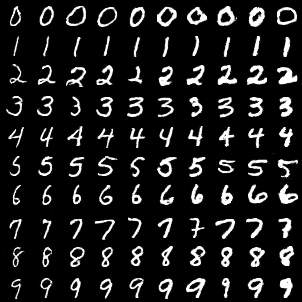
\includegraphics[width=\textwidth]{Img/icg-width.png}
    \caption{$c_2$调控生成数字的粗细}
    \label{ffig:m-icg-witdth}
  \end{subfigure} 
  \begin{subfigure}[b]{\trif\textwidth}
    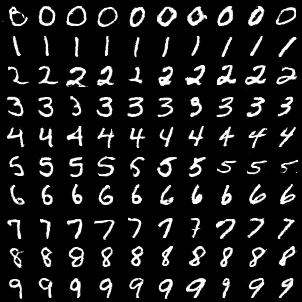
\includegraphics[width=\textwidth]{Img/icg-rotation.png}
    \caption{$c_3$调控生成数字的角度}
    \label{ffig:m-icg-rotation}
  \end{subfigure} 
  \begin{subfigure}[b]{\trif\textwidth}
    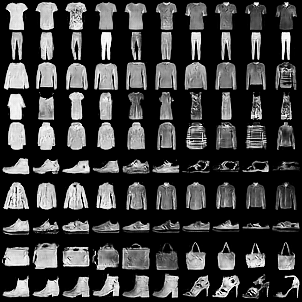
\includegraphics[width=\textwidth]{Img/icg-light.png}
    \caption{$c_2$调控生成图片的亮度}
    \label{ffig:fa-icg-light}
  \end{subfigure} 
  \caption{隐变量对生成图片的调控。图中每一行对应类别隐变量的一个取值,每一列对应其他某个隐变量(固定剩余隐变量)的连续变化。}
  \label{fig:latent-varies}
\end{figure}

\section{实现细节}
在实践中,模型中的所有模块(生成器、判别器、辅助网络等)均被实现为深度神经网络。具体实现可在Github上查看\footnote{实现代码地址:\url{https://github.com/guyueshui/baGAN}}。\textcolor{red}{网络结构在附录中给出。}

\subsection{C-InfoGAN}
对于C-InfoGAN模型,我们的设定和InfoGAN保持大致相同。辅助网络$Q$和判别器$D$共享大部分网络结构,$Q$在判别器的尾部(通常是倒数第二层)分离出一个全连接网络,输出后验概率的估计$Q(\bd{c}|\bd{x})$。因此,C-InfoGAN带来的计算复杂度增加较小。对于离散隐变量$c_i$,在输出之前施加一个softmax激活层,得到的输出代表$Q(c_i|\bd{x})$。对于连续隐变量$c_j$,我们假设其先验分布为高斯分布,然后利用$Q$网络输出它的均值和方差,放到高斯分布中去拟合,计算差值。
由于GAN在训练时容易坍塌,DCGAN\citep{radford2015unsupervised}提出了一种训练稳定的生成对抗网络结构,所以我们采用的网络结构对此有很多参考。关于超参数的选择我们也沿用InfoGAN的设定,对于离散隐变量设置为1;对于连续隐变量,设置为较小的值0.1。

表~\ref{tab:m-cig-netarch}是给出了C-InfoGAN在MNIST上的网络结构,如前所述,判别器$D$和辅助网络$Q$共享大部分网络结构。在MNIST数据集上,噪声空间的构成为一个10维离散隐变量,两个连续隐变量和62维高斯噪声,最终得到的噪声维度为74。对于FashionMNIST,我们在实践中发现使用同样的网络结构也能达到很好的效果。因此本文对于两个数据集采用同样的网络结构。
\begin{table}
  % \renewcommand\arraystretch{0.7} % set row height
  \centering
  \bicaption{C-InfoGAN在MNIST上的网络结构}
  {Architectures of C-InfoGAN used for MNSIT dataset}
  \begin{tabular}{l|l}
    \hline
    \textbf{生成器$G$}               & \textbf{判别器$D$/辅助网络$Q$} \\ \hline
    Input $\in \reals^{74}$          & Input $28\times 28$ Gray image \\ \hline
    fc 1024. bn. relu                & conv 64: k4, s2, p1. lrelu  \\ \hline
    fc $7\times7\times128$. bn. relu & conv 128: k4, s2, p1. bn. lrelu \\ \hline
    upconv 64: k4, s2, p1. bn. relu  & fc 1024. bn. lrelu \\ \hline
    upconv 1: k4, s2, p1. tanh       & fc 1. sigmoid. output for $D$, \\
    ~                                & fc 128. bn. lrelu. fc. output for $Q$ \\
    \hline
  \end{tabular}
  \label{tab:m-cig-netarch}
\end{table}

\subsection{InfoCatGAN}
对于InfoCatGAN,我采用的模型如下。
\begin{table}
  % \renewcommand\arraystretch{0.7} % set row height
  \centering
  \bicaption{InfoCatGAN在MNIST上的网络结构}
  {Architectures of InfoCatGAN used for MNSIT dataset}
  \begin{tabular}{l|l}
    \hline
    \textbf{生成器$G$}               & \textbf{判别器$D$} \\ \hline
    Input $\in \reals^{74}$          & Input $28\times 28$ Gray image \\ \hline
    fc 1024. bn. relu                & conv 64: k4, s2, p1. lrelu  \\ \hline
    fc $7\times7\times128$. bn. relu & conv 128: k4, s2, p1. bn. lrelu \\ \hline
    upconv 64: k4, s2, p1. bn. relu  & fc 1024. bn. lrelu \\ \hline
    upconv 1: k4, s2, p1. tanh       & fc 10. softmax \\
    \hline
  \end{tabular}
  \label{tab:m-icg-netarch}
\end{table}

\section{实验结果}

\subsection{MNIST}\label{sec:icg-ex}

图~\ref{ffig:m-cg}和图~\ref{ffig:m-icg}是在无监督情况下CatGAN和InfoCatGAN的生成效果,可以看到,InfoCatGAN的生成效果明显高于CatGAN,并且每一行基本是一种数字类别,对应隐变量的不同取值。半监督情况下有类似的结果,不同的是在少量标签信息的辅助下,InfoCatGAN可以将隐变量$c$和真实标签正确绑定,$c=1$对应生成数字`1',见图~\ref{ffig:m-ss-icg}。CatGAN生成的图片质量很差,原因在于其目标函数是为了分类而设计的。生成器的作用只是为了判别器能够更加鲁棒,如\ref{sec:icg-us}节所述,从\eqref{eq:catgan-g}式中可以看到,$G$的目标函数只有条件熵,无法针对性地生成图片,从而会降低生成图片的质量。而InfoCatGAN由于增加了隐变量$c$,并在训练过程中有意识地将生成数据的类别与之绑定,所以生成的图片质量较好。

\begin{figure}[htbp]
  \centering
  \begin{subfigure}[b]{\trif\textwidth}
    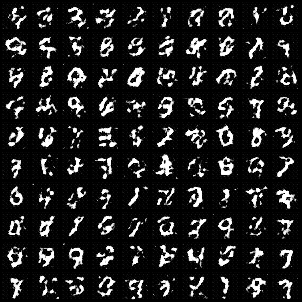
\includegraphics[width=\textwidth]{Img/cg.png}
    \caption{CatGAN}
    \label{ffig:m-cg}
  \end{subfigure}
  \begin{subfigure}[b]{\trif\textwidth}
    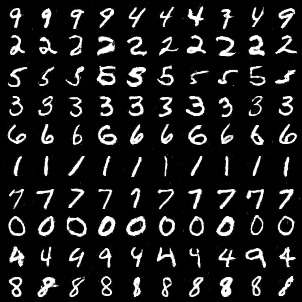
\includegraphics[width=\textwidth]{Img/icg.png}
    \caption{InfoCatGAN}
    \label{ffig:m-icg}
  \end{subfigure}
  \begin{subfigure}[b]{\trif\textwidth}
    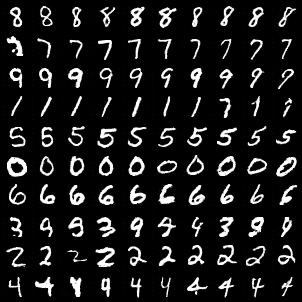
\includegraphics[width=\textwidth]{Img/ig.png}
    \caption{C-InfoGAN}
    \label{ffig:m-ig}
  \end{subfigure}

  \begin{subfigure}[b]{\trif\textwidth}
    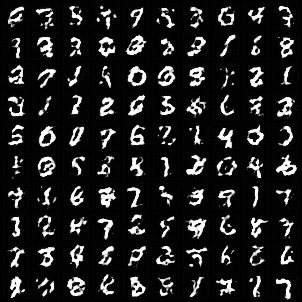
\includegraphics[width=\textwidth]{Img/cg-132labels.png}
    \caption{CatGAN(132 labels)}
    \label{ffig:m-ss-cg}
  \end{subfigure}
  \begin{subfigure}[b]{\trif\textwidth}
    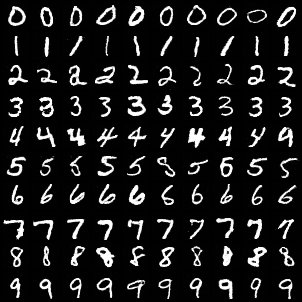
\includegraphics[width=\textwidth]{Img/icg-132labels.png}
    \caption{InfoCatGAN(132 labels)}
    \label{ffig:m-ss-icg}
  \end{subfigure}
  \begin{subfigure}[b]{\trif\textwidth}
    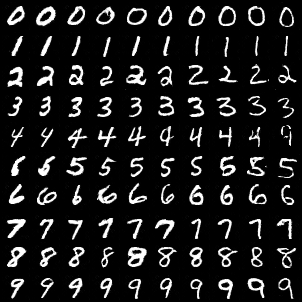
\includegraphics[width=\textwidth]{Img/ig-132labels.png}
    \caption{C-InfoGAN(132 labels)}
    \label{ffig:m-ss-ig}
  \end{subfigure}

  \caption{模型在MNIST上得生成效果。在InfoCatGAN和C-InfoGAN的生成结果中,每一行对应隐变量$c$的一个取值,从0到9。}
  \label{fig:mnist}
\end{figure}

表~\ref{tab:cat}给出了无监督和半监督情况下的分类准确率\footnote{表中有关CatGAN的数据来自与本文复现的结果,与\citet{springenberg2015unsupervised}有所差距。经过多次尝试,我们仍无法完美复现出原文中的结果。}。从表中看出,在无监督的情况下InfoCatGAN的分类准确率相较于CatGAN有所提升,而FID从236.75降低到8.04,图片生成质量有了极大的提升,见图~\ref{ffig:m-icg}。在半监督的情况下,CatGAN的准确率达到了96.05\%,而InfoCatGAN随着正则化系数$\lambda_1$的变化呈现出不同的效果。当系数较小时,分类准确率较高,但生成图片的质量非常差;当系数较大时,生成的图片效果很好,但分类准确率有所降低。通过调节参数$\lambda_1$,可以实现生成效果和分类准确率之间的折中。实验使用的默认值是$\lambda_1 = 1.1$,
当$\lambda_1$减小时,生成图片的质量开始下降,同时分类准确率也会相应增加。值得注意的是,$\lambda_1$越小并不意味着分类准确率越高。当$\lambda_1=0$时,InfoCatGAN退化为CatGAN;而从表~\ref{tab:cat}可以看出,当$\lambda_1=0.02$时,InfoCatGAN的分类准确率高于CatGAN,达到98.15\%。

\begin{table}[htbp]
  \centering
  \caption{MNIST分类准确率对比}
  \label{tab:cat}
  \begin{tabular}{|l|c|c|}
    \hline
    \textbf{模型} & \textbf{准确率(\%)} & \textbf{FID} \\
    \hline
    CatGAN & 64.41 & 236.75  \\ \hline
    InfoCatGAN & 69.04 & 8.04 \\ \hline
    C-InfoGAN & 77.65 & 7.55 \\ \hline
    CatGAN(132 labels) & 96.05 & 127.92 \\ \hline
    InfoCatGAN(132 labels, $\lambda_1 = 0.02$) & \textbf{98.15} & 169.72 \\ \hline
    InfoCatGAN(132 labels, $\lambda_1 = 0.03$) & 80.43 & \textbf{6.59} \\ \hline
    C-InfoGAN(132 labels) & 93.70 & 9.16 \\ \hline
  \end{tabular}
\end{table}

%\textcolor{red}{here begins c-infogan} 
图~\ref{ffig:m-ig}和图~\ref{ffig:m-ss-ig}给出了无监督和半监督情况下C-InfoGAN的生成结果。从图中可以看出无监督情况下,模型已经达到了很好的生成效果,隐变量$c$基本可以控制生成图片的类别,但是仍有部分类别未能精确控制(图~\ref{ffig:m-ig});在半监督情况下,隐变量达到了精确的绑定,每一行对应生成一种类别的数字,而且顺序和真实标签是对应的。另外从图~\ref{fig:latent-varies}可以看出,C-InfoGAN模型不仅可以生成指定类别的图片,并且可以通过额外的隐变量调节图片局部特征,如手写数字的粗细,角度等,这对指定特征的数据补足具有很大意义。

表~\ref{tab:cat}给出了C-InfoGAN的准确率和FID及其与CatGAN模型的性能对比。可以看出,相较于CatGAN模型,C-InfoGAN模型可以获得更高的准确率和生成质量,而且隐变量的绑定效果也更好。而在半监督情况下,C-InfoGAN在保证生成质量的前提下,仍然能够达到93.7\%的分类准确率。这是因为InfoGAN模型使用的是一个辅助网络$Q$来做类别绑定和分类任务,训练过程中并没有判别器做过多约束,所以无论如何调整分类网络或更改分类约束,也不会对生成效果产生很大影响。这使得模型可以进一步利用生成的图片和标签扩充数据集,以达到更进一步的性能提升。

\subsection{FashionMNIST}\label{sec:fashion}

FashionMNIST\citep{xiao2017/online}是一个类似MNIST的数据集,二者拥有同样的结构,图像大小,同样的类别数目。但是相对于MNIST,FashionMNIST拥有更复杂的图像结构,以及更难获得非常高的分类准确率,所以对模型更具有检验性。

表~\ref{tab:fashion}给出了模型在FashionMNIST的数值结果,其中InfoCatGAN的正则系数$\lambda_1 = 0.03$。从表中可以看出,无论是在无监督还是半监督情况下,CatGAN的分类准确率都是比较高的,但从生成效果来看,它却是最差的。在无监督情况下,InfoCatGAN提高了生成图片的质量,但与此同时,牺牲了分类准确率,而C-InfoGAN在一定程度上二者兼顾,不仅生成质量最优,而且具有相对较高的分类准确率,此外其模型复杂度也较低。在半监督情况下,InfoCatGAN在两个方面均体现出优势,分类准确率达到了74.21\%,FID为$16.92$,生成效果见图~\ref{ffig:ss-icg},这说明增加标签信息对模型的增益很大。

\begin{table}[htbp]
  \centering
  \caption{FashionMNIST分类准确率对比}
  \label{tab:fashion}
  \begin{tabular}{|l|c|c|}
    \hline
    \textbf{模型} & \textbf{准确率(\%)} & \textbf{FID} \\
    \hline
    CatGAN & 64.28 & 120.04  \\ \hline
    InfoCatGAN & 57.66 & 26.43 \\ \hline
    C-InfoGAN & 60.50 & 15.97 \\ \hline
    CatGAN(100 labels) & 73.34 & 119.16 \\ \hline
    InfoCatGAN(100 labels) & \textbf{74.21} & 16.92 \\ \hline
    C-InfoGAN(100 labels) & 68.94 & \textbf{15.94} \\ \hline
  \end{tabular}
\end{table}

\begin{figure}[htbp]
  \centering
  \begin{subfigure}[b]{\trif\textwidth}
    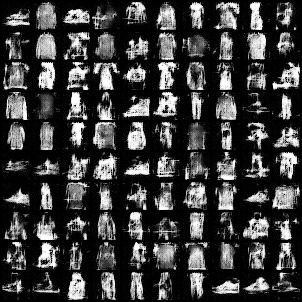
\includegraphics[width=\textwidth]{Img/fa-cg.png}
    \caption{CatGAN}
  \end{subfigure}
  \begin{subfigure}[b]{\trif\textwidth}
    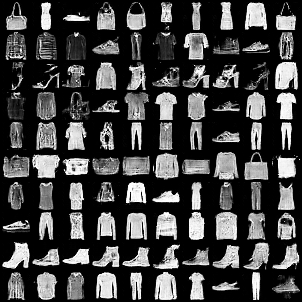
\includegraphics[width=\textwidth]{Img/fa-icg.png}
    \caption{InfoCatGAN}
  \end{subfigure}
  \begin{subfigure}[b]{\trif\textwidth}
    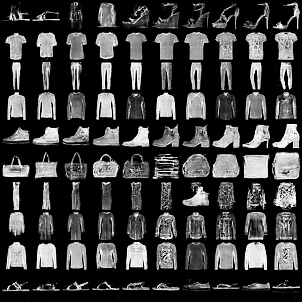
\includegraphics[width=\textwidth]{Img/fa-ig.png}
    \caption{C-InfoGAN}
  \end{subfigure}

  \begin{subfigure}[b]{\trif\textwidth}
    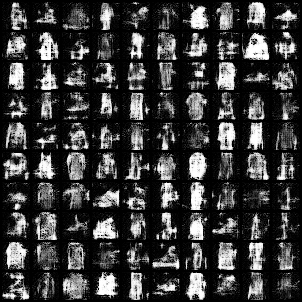
\includegraphics[width=\textwidth]{Img/fa-cg-100labels.png}
    \caption{CatGAN(100 labels)}
  \end{subfigure}
  \begin{subfigure}[b]{\trif\textwidth}
    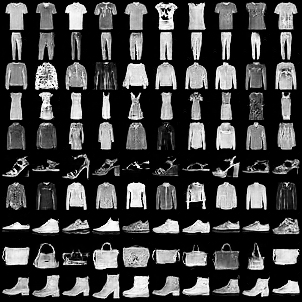
\includegraphics[width=\textwidth]{Img/fa-icg-100labels.png}
    \caption{InfoCatGAN(100 labels)}
    \label{ffig:ss-icg}
  \end{subfigure}
  \begin{subfigure}[b]{\trif\textwidth}
    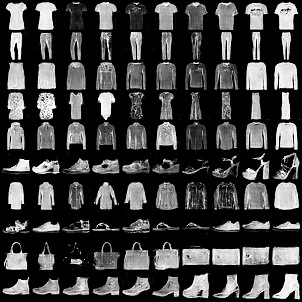
\includegraphics[width=\textwidth]{Img/fa-ig-100labels.png}
    \caption{C-InfoGAN(100 labels)}
    \label{ffig:ss-ig}
  \end{subfigure}

  \caption{模型在FashionMNIST上的生成效果。在InfoCatGAN和C-InfoGAN的生成结果中,每一行对应隐变量$c$的一个取值,从0到9。}
  \label{fig:fashion}
\end{figure}

图~\ref{fig:fashion}中给出了所有模型的生成结果。值得一提的是,加入互信息约束后的半监督版本模型从上往下每一行都对应同一个类别,并且顺序和训练数据的真实标签正确对应(图~\ref{ffig:ss-icg}、\ref{ffig:ss-ig})。这说明了隐变量正确绑定到类别特征,并且可以精准调控生成图片的类别。

\subsection{收敛速度分析}
本文提出的两个模型在原理上都属于正则化生成对抗网络,因此相较于原先的两个模型CatGAN和InfoGAN,增加的计算复杂度很小。由于GAN的训练方式特殊,训练的过程是生成器和判别器的对抗,因此目前没有一个统一的评判收敛性的标准。针对InfoCatGAN和C-InfoGAN两种模型,本文分别用条件熵损失(即判别器输出的概率分布对应的熵)以及互信息损失(实际采用交叉熵估计,详见\ref{sec:cig-us}节)来作为模型收敛的佐证,见图~\ref{fig:convergence}。
\begin{figure}[htbp]
  \centering
  \begin{subfigure}[b]{\twof\textwidth}
    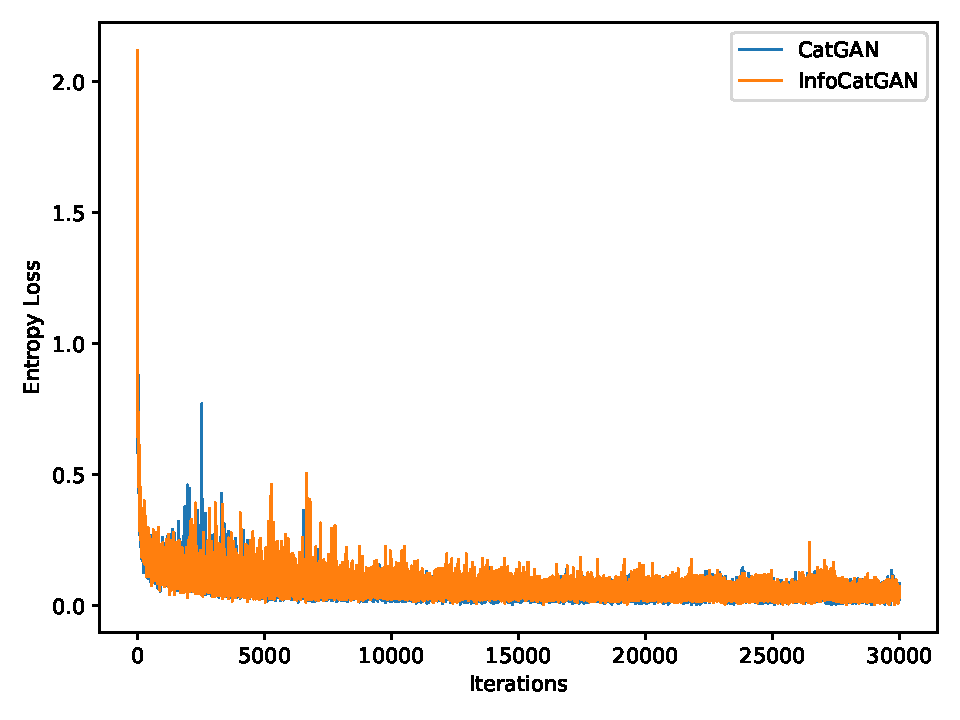
\includegraphics[width=\textwidth]{Img/icg-convergence.pdf}
    \caption{Entropy loss of CatGAN and InfoCatGAN}
    \label{ffig:icg-convergence}
  \end{subfigure}
  \begin{subfigure}[b]{\twof\textwidth}
    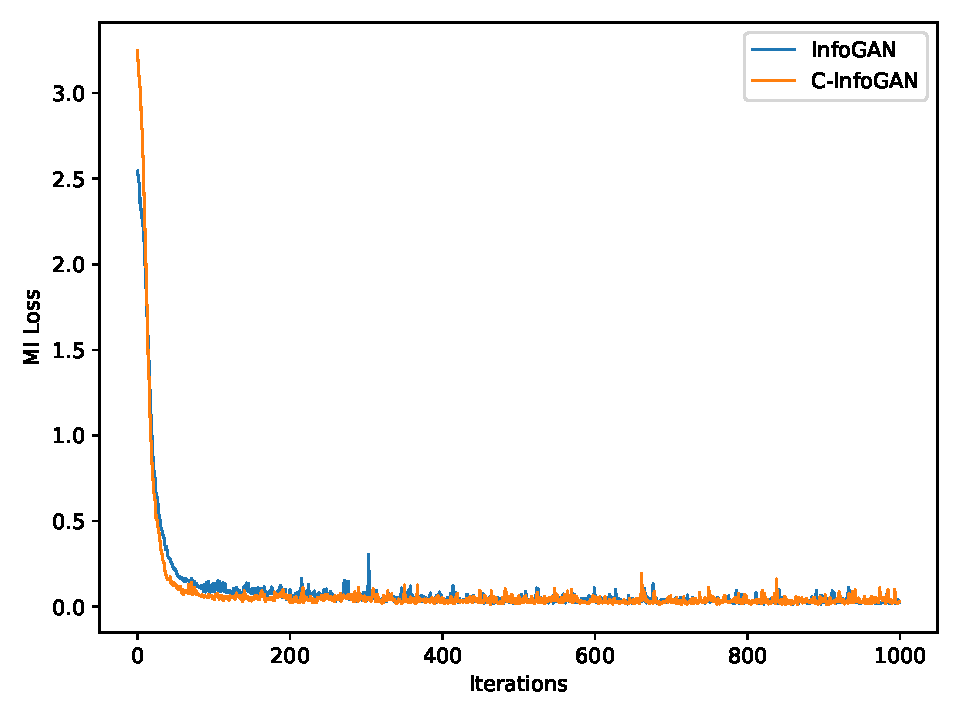
\includegraphics[width=\textwidth]{Img/cig-convergence.pdf}
    \caption{Mutual information loss of InfoGAN and C-InfoGAN}
    \label{ffig:cig-convergence}
  \end{subfigure}
  \bicaption{模型在MNIST上的收敛速度}{Convergence speed on MNIST}
  \label{fig:convergence}
\end{figure}